\section{\secrecseq}
\label{sec_recursively_defined_sequences}

In \Cref{sec_explicitly_defined_sequences}, we looked at sequences defined by an explicit rule.  Another way of defining a sequence uses a recursive rule in which each term is defined in terms of the previous term(s).  In this section, we evaluate recursively-defined sequences and model with recursively-defined sequences. But first, we start with an activity.

%%%%%%%%%%%%%%%%%%%%%%%%

\newcommand{\subhanoi}{The Towers of Hanoi}
\subsection{\subhanoi}
\label{sub_towers_hanoi}

The puzzle we are about to do is famous.  Do not look for information about it online -- that will spoil the fun.

\begin{act}[Towers of Hanoi Puzzle]
\label{act_hanoi}
~
    Given a disks of various diameters stacked in order on the first of three towers (pegs) as shown in \Cref{fig_hanoi_start_end}, it is only physically possible to lift the top disk up off any peg and put it down on another peg.  Your goal is to move the entire tower of disks from the first tower to the third tower subject to two rules:

        \begin{description}
            \item[\quad Rule 1:] You may only move one disk at a time.
            \item[\quad Rule 2:] You may not put a larger disk on top of a smaller one.
        \end{description}

        \begin{figure}[hbtp]
            \centering
            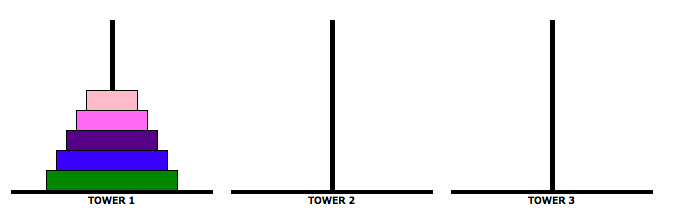
\includegraphics[width=0.5\linewidth]{Puzzles/Puzzle_Images/TowerHanoiStart.png}
            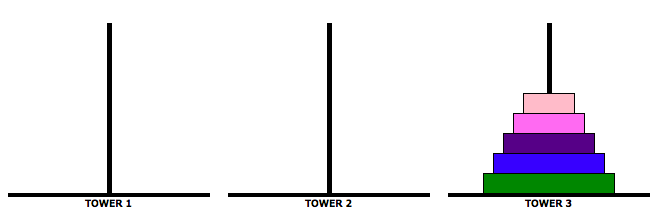
\includegraphics[width=0.5\linewidth]{Puzzles/Puzzle_Images/TowerHanoiEnd.png}
            \caption{The starting and end configurations for the Towers of Hanoi game.}
            \label{fig_hanoi_start_end}
        \end{figure}

        \begin{actpart}
            \item \label{part_hanoi3} Go to \url{\http://www.dynamicdrive.com/dynamicindex12/towerhanoi.htm} to play the Towers of Hanoi game. You can move a disk by clicking on it and dragging it to another peg.  Solve the puzzle for three disks.
            \item Solve the puzzle for four disks without using the solve button.
            \item Now, use the solve button to solve the puzzle for four disks.  Keep track of when and where the largest disk moves.  Where are the other disks when it moves? Hint: The largest disk moves once.  
            \item \label{part_hanoi_3to4} The minimum number of moves to solve the puzzle with three disks is seven. To solve the puzzle for four disks we need to move the top three disks, then the largest disk, and then we need to move the top three disks again.  Explain why this strategy gives a solution to the puzzle with four disks in $$7+1+7=15$$ moves.
            \item Use the solve button to solve the puzzle for four disks again and look for the minimum number of moves. 
            \item \label{part_hanoi_guess5} Generalize our strategy from (\ref{part_hanoi_3to4}) to guess how many moves it will take to solve the puzzle with five disks.
            \item Use the solve button to check your answer to (\ref{part_hanoi_guess5}).
            \item Consider the sequence $h$ where $h_n$ is the minimum number of moves needed to solve the puzzle with $n$ disks for $n \ge 1$.  The minimum number of moves needed to solve the puzzle with $n-1$ disks would then be $h_{n-1}$.  Make a conjecture about a rule for $h_n$ in terms of $h_{n-1}$.
            \item \label{part_hanoi_terms} We saw that $h_3=7$, $h_4=15$, and $h_5=31$.  Use the solve button to calculate $h_6$ and $h_7$.  
            \item Based on the numbers from (\ref{part_hanoi_terms}), make a conjecture about an explicit rule for $h_n$.
        \end{actpart}
\end{act}

Let's take a closer look at \Cref{act_hanoi}.  

\begin{exam}[Tower of Hanoi puzzle]
\label{exam_hanoi_recursion}
    Consider the sequence $h$ where $h_n$ is the minimum number of moves needed to solve the puzzle with $n$ disks for $n \ge 1$.  The minimum number of moves needed to solve the puzzle with $n-1$ disks would then be $h_{n-1}$.  Make a conjecture about a rule for $h_n$ in terms of $h_{n-1}$.
        \begin{soln}
            To solve the puzzle for $n$ disks, we can break the process into three phases.  
                \begin{description}
                    \item [\quad Phase 1] Relocate the top $n-1$ disks in the pile to Tower 2.  [$h_{n-1}$ moves]
                    \item [\quad Phase 2] Move the largest disk to Tower 3.  [1 move]
                    \item [\quad Phase 3] Relocate the top $n-1$ disks in the pile to Tower 3.  [$h_{n-1}$ moves]
                \end{description}
            This analysis tells us that $$h_n=2h_{n-1}+1.$$
        \end{soln}
\end{exam}

%%%%%%%%%%%%%%%%%%%%%%%%

\newcommand{\subrecdefseq}{Recursively-defined Sequences}
\subsection{\subrecdefseq}
\label{sub_seq_recursive}

In \Cref{sec_explicitly_defined_sequences}, we worked with sequences that were defined explicitly, by a formula or in words. Let's take a closer look at two of those sequences.

\begin{exam}[First look at recursively-defined sequences]
\label{exam_first_look_rec_seq} 
~
    \begin{apart}
        \item Consider the sequence $a_n$ from \Cref{act_eval_seq} that was defined by $a_n=10n+2$ for $n\ge 0$.  The first few terms are $$2, 12, 32, 42, 52, \ldots.$$ What do we notice about how each term is calculated from the previous term?
            \begin{soln}
                Each term ($a_n$) is ten more than the previous term ($a_{n-1}$) .  That is,          
                    $$2 \xrightarrow[+ 10]{} 12 \xrightarrow[+ 10]{} 22 \xrightarrow[+ 10]{} 32 \xrightarrow[+ 10]{} 42 \xrightarrow[+ 10]{} 52.$$
                Thus for $n\ge 1$ we have $$a_n=a_{n-1}+10.$$
            \end{soln}
        \item Consider the sequence $b_i$ from \Cref{act_eval_seq} that was defined by $b_i=2\cdot10^i$ for $i\ge 0$. The first few terms are $$2, 20,200,2000,20000, \ldots.$$ What do we notice about how each term is calculated from the previous term?
            \begin{soln}
                Each term ($b_i$) is ten times the previous term ($b_{i-1}$).  That is,         
                    $$2 \xrightarrow[\times 10]{} 20 \xrightarrow[\times 10]{} 200 \xrightarrow[\times 10]{} 2000 \xrightarrow[\times 10]{} 20000.$$
                Thus for $i\ge 1$ we have $$b_i=10b_{i-1}.$$
            \end{soln} 
    \end{apart}
\end{exam} 

Let's look at a sequence defined by such a rule.

\begin{exam}[Double and add three]
\label{exam_double_and_add3}
    Consider the sequence $c$ is defined by the $c_0=1$ and $$c_k=2c_{k-1}+3$$
    for $k \ge 1$.  Note that the rule for this sequence is actually piecewise-defined
        $$c_k = \left\{\begin{array}{cl}
        1 & \text{if } k=0 \\
        2c_{k-1}+3 & \text{if } k\ge 1 \end{array} \right.$$
    Also notice that the second part of the rule gives an infinite list of equations:
        \begin{align*}
            (k=1) \quad c_1&=2c_0+3 \\
            (k=2) \quad c_2&=2c_1+3 \\
            (k=3) \quad c_3&=2c_2+3 \\
            (k=4) \quad c_4&=2c_3+3 \\
            & \vdots
        \end{align*}
        It is often helpful to think of the rule in words
            \begin{center}
                To get each term, we double the previous term and then add 3.
            \end{center}
    \begin{actpart}
        \item Evaluate $c_4$.
            \begin{soln}
                First recall that $c_0=1$.  When $k=1$ the rule tells us
                    $$c_1=2c_0+3=2(1)+3=5.$$
                Next, when $k=2$ we get
                    $$c_2=2c_1+3=2(5)+3=13.$$
                When $k=3$ we have
                    $$c_3=2c_2+3=2(13)+3 = 29.$$
                Finally, when $k=4$ we find
                    $$c_4=2c_3+3=2(29)+3=61.$$   
            \end{soln}
        \item Write an explicit rule for $c_k$.  
            \begin{soln}
                Since we are multiplying the previous term by 2 each time, it is reasonable to suspect that an explicit formula involves a power of 2. \Cref{table_exam_double_and_add3} compares the first five terms of $c$ to the powers of 2. Since there is no obvious pattern with $2^k$ we have listed $2^{k+1}$ and then $2^{k+2}$ as well. It looks like $c_k$ is 3 smaller than $2^{k+2}$ and so we conjecture that $c_k=2^{k+2}-3$. 

                We can check that the definition gives $c_5=2c_4+3=2(61)+3 = 125$ and our explicit formula gives $c_5=2^{5+2}-3 = 128-3 = 125$. We will see how to verify these conjectures in \Cref{sec_math_ind}.
                \begin{table}[hbtp]
                        \centering
                        \begin{tabular}{c|c |c|c |c|c}
                            $k$ & 0 & 1 & 2 & 3 & 4  \\ \hline
                            $c_k$ & 1 & 5 & 13 & 29 & 61 \\ \hline
                            $2^k$ & 1 & 2 & 4 & 8 & 16  \\ \hline
                            $2^{k+1}$ & 2 & 4 & 8 & 16 & 32 \\ \hline
                            $2^{k+2}$ & 4 & 8 & 16 & 32 & 64 \\
                        \end{tabular}
                        \caption{The terms of the sequence from \Cref{exam_double_and_add3} compared to the powers of 2.}              \label{table_exam_double_and_add3}
                    \end{table}
            \end{soln}
        \end{actpart}
\end{exam}

We state the formal definitions.

\begin{defn}[Recursively-defined sequence]
~
    \begin{apart}
        \item The first term (or first few terms) of a sequence is the \vocab{initial condition(s)}.  If a sequence $a$ starts at $s$ for some nonnegative integer $s$, then the initial condition is $a_s$ (and perhaps subsequent terms such as $a_{s+1}$, $a_{s+2}$, etc.)  For example, the initial condition for the sequence $c$ defined in \Cref{exam_double_and_add3} was $c_0=1$.
        \item A \vocab{recursion} (or \vocab{recursive rule}) for a sequence specifies how each term ($a_n$) can be calculated from the previous term(s) ($a_{n-1}$ and perhaps $a_{n-2}$, $a_{n-3}$, and so on). For example, the recursion for the sequence $c$ defined in \Cref{exam_double_and_add3} was $c_n=2c_{n-1}+3$.  A recursion may involve the index $n$ as well as previous term(s). A recursion should use the previous term(s) in a nontrivial way. We do not consider explicitly-defined rules (that use the index but not previous terms) to be recursive.
        \item A sequence is \textbf{recursively-defined} if we are given a recursion and enough initial conditions to evaluate the recursion at all values.  For example, the recursion for the sequence $c$ defined in \Cref{exam_double_and_add3} starts at $k=1$, so we needed the initial condition to provide the value of $c_0$.
        \item A recursive rule that involves only one previous term is \vocab{first order}.  For example, the sequence $c$ defined in \Cref{exam_double_and_add3} is first-order.
    \end{apart}
\end{defn}

Now it is your turn to work with recursively-defined sequences.

\begin{act}[Evaluating recursively-defined sequences]
\label{act_eval_rec_def_seq}
~
    \begin{actpart}
        \item Evaluate the first four terms of the sequence defined by $t_0=3$ and $t_i=3t_{i-1}-5$ for $i \ge 1$.  %ans 3, 4, 7, 16
        %\item Evaluate the first four terms of the sequence defined by $u_1=5$ and $u_k=-2u_{k-1}$ for $k \ge 2$.
        \item Evaluate $v_3$ for the sequence defined by $v_0=2$ and $v_m=v_{m-1}^2-1$ for $m \ge 1$. % ans 2, 3, 8, 63
        \item Evaluate $a_5$ for the sequence defined by $a_1 = 5$ and $a_n=a_{n-1}+2n$ for $n\ge 2$.  Note that the recursion involves the index $n$.  For example, when $n=2$ we get $a_2=a_1+2(2)=5+4=9$ and when $n=3$ we have $a_3=a_2+2(3)=9+6=15.$
        \item Evaluate $b_4$ for the sequence defined by $b_1=1$ and $b_k=kb_{k-1}$ for $k \ge 2$.  What do you notice? Write an explicit formula for $b_k$.
        \item Evaluate $c_4$ for the sequence defined by $c_0=0$ and $c_i=c_{i-1}+i$ for $i \ge 1$. What do you notice?  Write an explicit formula for $c_i$. Hint: Handshakes.
    \end{actpart}
\end{act}

As we saw in \Cref{act_eval_rec_def_seq}, a recursion can involve the index.  Let's look at some similar examples.

\begin{exam}[Evaluating recursively-defined sequences that involve the index]
\label{exam_eval_rec_def_seq_involving_index}
~
    \begin{apart}
        \item Evaluate $d_5$ for the sequence defined by $d_1 = 1$ and $d_n=d_{n-1}+2n-1$ for $n\ge 2$. What do you notice?  Write an explicit formula for $d_n$.
            \begin{soln}
                When $n=2$, we have $d_2=d_1+2(2)-1=1+3=4$. 
                
                When $n=3$, we have $d_3=d_2+2(3)-1=4+5=9.$
                
                When $n=4$, we have $d_4=d_3+2(4)-1=9+7=16.$
                
                When $n=5$, we have $d_5=d_4+2(5)-1=16+9 = 25.$

                Notice $d_1=1 = 1^2$, $d_2=4=2^2$, $d_3=9=3^2$, $d_4=16=4^2$, and $d_5=25=5^2$.  
                
                We conjecture that $d_n=n^2$ for $n \ge 1$.
            \end{soln}
        \item Evaluate $s_4$ for the sequence defined by $s_1=10$ and $s_k=ks_{k-1}$ for $k \ge 2$.  What do you notice? Write an explicit formula for $b_k$.
            \begin{soln}
                When $k=2$, we have $s_2=sb_1 = 2(10) = 20$.
                
                When $k=3$, we have $s_3=3s_2 = 3(20) = 60$.
                
                When $k=4$, we have $s_4=4s_3 = 4(60) = 240$.

                Notice that $s_1=10=10(1!)$, $s_2=20=10(2!)$, 
                $s_3=60=10(3!)$,
                and $s_4=240=10(4!)$.  

                We conjecture that $s_k=10(k!)=10k!$
            \end{soln}
            \item Evaluate $t_4$ for the sequence defined by $t_0=0$ and $t_i=t_{i-1}+2i$ for $i \ge 1$. What do you notice?  Write an explicit formula for $t_i$. Hint: Factor.
                \begin{soln}
                    When $i=1$, we have $t_1=t_0+2(1) = 0+2=2$.

                    When $i=2$, we have $t_2=t_1+2(2) = 2+4=6$.

                    When $i=3$, we have $t_3=t_2+2(3) = 6+6=12$.

                    When $i=4$, we have $t_4=t_3+2(4) = 12+8=20$.

                    Notice that $t_0=0=(0)(1)$, $t_1=2=(1)(2)$, $t_2=6=(2)(3)$, $t_3=12=(3)(4)$,  and $t_4=20=(4)(5)$.  

                    We conjecture that $t_i=i(i+1)$ for $i \ge 0$.
                \end{soln}
    \end{apart}
\end{exam}
        
%%%%%%%%%%%%%%%%%%%%%%%%

\newcommand{\subntr}{Modeling with Recursively-defined Sequences}
\subsection{\subntr}
\label{sub_next_term_recursive}

In the examples we have seen so far, we have gone from a sequence defined recursively  to a list of terms or explicitly-defined rule.  It is particularly useful to go the opposite direction, from a list or explicitly-defined rule to a recursively-defined sequence.  Let's try modeling with such sequences.

\begin{exam}[Write the recursive rule for sequence from list]
\label{exam_write_rec_from_list}
~    
    \begin{apart}
        \item Write a simple recursive rule that generates a sequence $a$ that begins
        $$5, 6, 7, 8, 9, 10, \ldots$$
            \begin{soln}
                To get from each term to the next we add 1. That is,         
                    $$5 \xrightarrow[+ 1]{} 6 \xrightarrow[+ 1]{} 7 \xrightarrow[+ 1]{} 8 \xrightarrow[+ 1]{} 9 \xrightarrow[+ 1]{} 10.$$
                Thus $a_0=5$ and $a_n=a_{n-1}+1$ for $n \ge 1$.
                By the way, an explicit rule for this sequence is $a_n=n+5$ for $n\ge 0$.
            \end{soln}

        \item Write a simple recursive rule that generates a sequence $b_n$ defined by $b_n=(n+1)(2n+1)$ for $n \ge 0$. Hint: The recursive definition depends on the index as well as the previous term.  
        \begin{soln}
            Let's find the first few terms of $b$. We get $b_0 = (1)(1) = 1$, 
            $b_1 = (2)(3) = 6$,
            $b_3 = (4)(7) = 28$,
            $b_4 = (5)(9) = 45$, and
            $b_5 = (6)(11) = 66$.  
            That is, the sequence $b$ begins $$1, 6, 15, 28, 45, 66, \ldots $$  

            Look at what we add to get each term from the previous term:
            $$1 \xrightarrow[+ 5]{} 6
            \xrightarrow[+ 9]{} 15
            \xrightarrow[+ 13]{} 28
            \xrightarrow[+ 17]{} 45
            \xrightarrow[+ 21]{} 66.$$
            The values we are adding 
                $$5,9,13,17,21,\ldots$$
            appear to depend on the index.  An explicit rule for these terms we are adding is $4n+1$ for $n \ge 1$.  A recursive rule is $b_0=1$ and $$b_n=b_{n-1}+4n+1$$ for $n \ge 1$.  
        \end{soln}
    \end{apart}   
\end{exam}

Try writing recursive definitions.

\begin{act}[Modeling with recursively-defined sequences]
\label{act_next_term_rec}
    Write a simple recursive rule that generates each sequence. Make sure you state where the index starts and include the initial condition.  Start your indexing at 0 or 1 (your choice). 
        \begin{actpart}
            \item $1, 6, 11, 16, 21, \ldots$ 
            \item $2, -10, 50, -250, 1250,\ldots$ 
            
            \item $2, \frac{1}{2}, 2, \frac{1}{2}, 2, \frac{1}{2}, \ldots$
            \item $5, 10, 30, 120, 600, \ldots$   Hint: What do we multiply by to get from each term to the next?  Write a recursion that involves the index.
            \item $5, 9, 17, 33, 65, 129, \ldots$. Write a recursion that does not involve the index. Hint: The recursion begins by doubling the previous term.
            \item $5, 9, 17, 33, 65, 129, \ldots$. Now write a recursion that involves the index. 
        \end{actpart}
\end{act}

Let's look at more examples writing the recursion from a list.

\begin{exam}[Modeling with recursively-defined sequences]
\label{exam_next_term_recursive}
    Write a simple recursive rule that generates each sequence. Make sure you state where the index starts and include the initial condition.  Start your indexing at 0 or 1 (your choice). 
        \begin{apart}
            \item $3, 6, 18, 72, 360, \ldots$   Write a recursion that involves the index.
                \begin{soln}
                    Look at what we multiply by to get each term from the previous term:
                        $$3 \xrightarrow[\times 2]{} 6
                        \xrightarrow[\times 3]{} 18
                        \xrightarrow[\times 4]{} 72
                        \xrightarrow[\times 5]{} 360.$$
                    If we set $a_1=3$, then $a_2=6 =2(3)=2a_1$, $a_3=18 =3(6)=3a_2$, $a_4=72 =4(18)=4a_3$, and $a_5=360 =5(72)=5a_4$.

                    We conjecture that $a_1=$ and $a_n=na_{n-1}$ for $n \ge 2$.
                \end{soln}
            \item $4, 7, 13, 25, 49, 97, \ldots$. Write a recursion that does not involve the index. Hint: The recursion begins by doubling the previous term.
                \begin{soln}
                    Let's set $b_0 = 4$.  Notice that $b_1=7 = 2(4)-1=2b_0-1$, $b_2=13 = 2(7)-1=2b_1-1$, $b_3=25 = 2(13)-1=2b_2-1$,  $b_4=49 = 2(25)-1=2b_3-1$, and $b_5=97 = 2(49)-1=2b_4-1$.  We conjecture that $b_0 = 4$ and $b_n=2b_{n-1}-1$ for $n \ge 1$.
                \end{soln}
            \item $4, 7, 13, 25, 49, 97, \ldots$. Now write a recursion that involves the index. 
                \begin{soln}
                     Look at what we add to get each term from the previous term:
                        $$4 \xrightarrow[+ 3]{} 7
                        \xrightarrow[+ 6]{} 13
                        \xrightarrow[+ 12]{} 25
                        \xrightarrow[+ 24]{} 49
                        \xrightarrow[+ 48]{} 97.$$
                     The terms we added are $3, 6, 12, 24, 48, \ldots$.  Each integer we added is twice the previous integer, so an explicit form is $3\cdot 2^n$ for $n \ge 0$.  That is, we have 
                        $$4 \xrightarrow[+ 3\cdot 2^0]{} 7
                        \xrightarrow[+ 3\cdot 2^1]{} 13
                        \xrightarrow[+ 3\cdot 2^2]{} 25
                        \xrightarrow[+ 3\cdot 2^3]{} 49
                        \xrightarrow[+ 3\cdot 2^4]{} 97.$$

                    Thus, we have $b_0=4$, $b_1 = 7 = 4+ 3\cdot 2^0$, $b_2 = 13 = 7+ 3\cdot 2^1$, $b_3 = 25 = 13+ 3\cdot 2^2$, $b_4 = 49 = 25+ 3\cdot 2^3$, and $b_5 = 97 = 49+ 3\cdot 2^4$.

                     We conjecture that $b_0=4$ and $b_n=b_{n-1}+3\cdot2^{n-1}$ for $n \ge 1$.
                \end{soln}
        \end{apart}
\end{exam}

%%%%%%%%%%%%%%%%%%%%%%%%

\subsection{Exercises}

%%%%%%%%%%%%%%%%%%%%%%%%

\subsubsection*{Exercises for \Cref{sub_towers_hanoi}
 \subhanoi}

\begin{exer}[\exerP] % Tower of Hanoi 8-9 disks
\label{exer_hanoi89}
~
    \begin{exerpart}
        \item \label{part_hanoi8} Use the recursion from \Cref{exam_hanoi_recursion} to calculate the minimum number of moves needed to solve the Tower of Hanoi puzzle with 2, 3, 4, 5, 6, 7, 8 disks.  Hint: It takes one move to solve the puzzle with one disk.
        \item Go to \url{\http://www.dynamicdrive.com/dynamicindex12/towerhanoi.htm} and watch the solution for eight disks.  Does the minimum number of moves agree with your answer to (\ref{part_hanoi8})?
        \item What is the minimum number of moves needed to solve the Tower of Hanoi puzzle with nine disks?  Explain how to use the recursion to answer.
    \end{exerpart}
\end{exer}

\begin{exer}[\exerU] % explicit formula Tower of Hanoi
\label{exer_hanoi_explicit}
    Let $h_n$ be the minimum number of moves needed to solve the Tower of Hanoi puzzle with $n$ disks.
    \begin{exerpart}
        \item List the first eight terms of $h_n$ from our work on \Cref{act_hanoi} or \Cref{exer_hanoi89}.
        \item Conjecture an explicit formula for $h_n$.  
        \item Use the explicit formula to calculate $h_9$ and $h_{10}$.
    \end{exerpart}
\end{exer}

\begin{exer}[\exerU] % can always solve Tower of Hanoi puzzle
\label{exer_hanoi_exist_soln}
   Use the phases discussed in \Cref{exam_hanoi_recursion} to explain why there exists a solution to the Tower of Hanoi puzzle for any number of disks.
\end{exer}

\begin{exer}[\exerU] % labeling states in Tower of Hanoi
\label{exer_hanoi_label_states}
    In the Tower of Hanoi puzzle, label the towers 1, 2, and 3.  An arrangement of $n$ disks can be represented by the $n-tuple$
    $$(a_1,a_2,\ldots, a_{n-1}, a_n)$$
    where $a_1$ is the tower number of the largest disk, $a_2$ is the tower number of the next largest disk, \ldots, $a_{n-1}$ is the tower number of the next-to-smallest disk, and $a_n$ is the tower number of the smallest disk.  In this notation, the starting state is $(1,1,\ldots, 1,1)$ and the ending state is $(2,2,\ldots, 2,2)$.  
        \begin{exerpart}
            \item Represent the state in \Cref{fig_hanoi5} with a 5-tuple.

            \begin{figure}[hbtp]
                \centering
                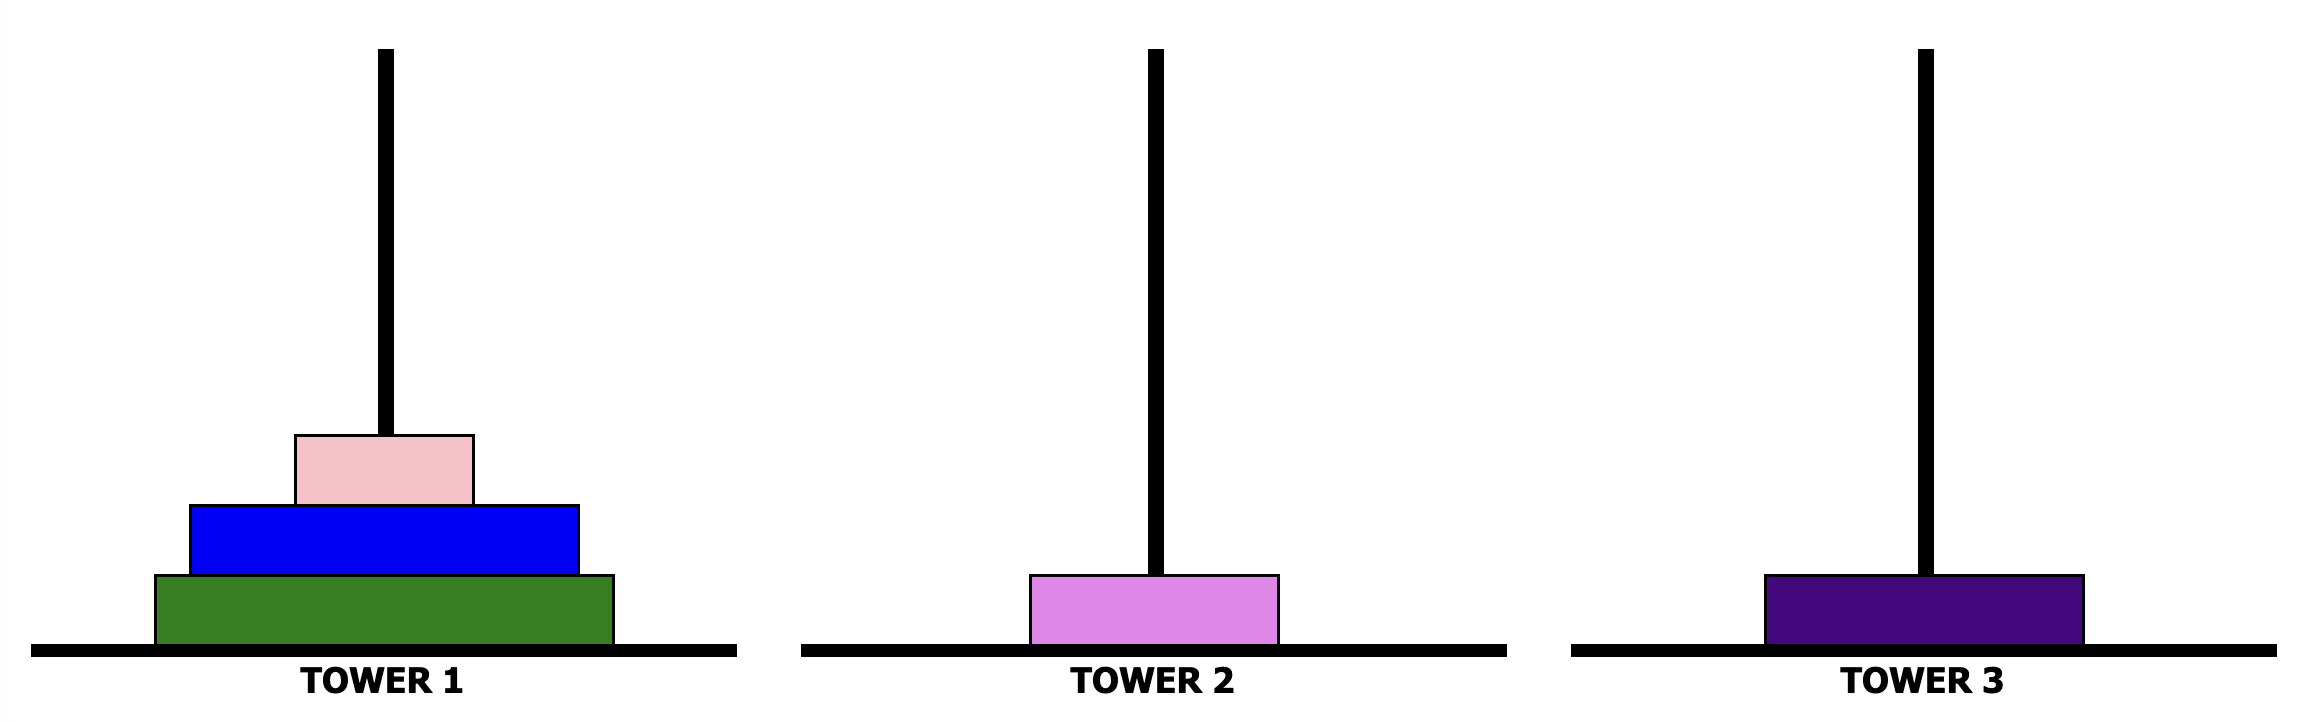
\includegraphics[width=0.5\linewidth]{Images/Hanoi_state.png}
                \caption{A state of the Tower of Hanoi puzzle with five disks.}
                \label{fig_hanoi5}
            \end{figure}
            \item List the states in a minimal solution of the Tower of Hanoi with three disks.  
            \item How many possible states are there in the Tower of Hanoi with three disks?  Explain how you counted.
            \item Explain why each tuple uniquely determines a state. That is, this representation is a pairing between the states of the Tower of Hanoi puzzle and the elements of $\{1,2,3\}^3$.  
        \end{exerpart}
\end{exer}

\begin{exer}[\exerE] % drawing Graphs of Hanoi
\label{exer_hanoi_graphs}
    In this problem we introduce the \vocab{graph of Hanoi}. $H_3$ which has a vertex for each possible state.  As we saw in \Cref{exer_hanoi_label_states}, each state corresponds to a unique $3$-tuple in $\{1,2,3\}^3$.  There is an edge between two vertices in $H_33$ if we can move between those two states with a single move in the puzzle. For example, there is an edge between $(1,1,1)$ and $(1,1,2)$ corresponding to moving the smallest disk from tower 1 to tower 2 and there is an edge between $(1,2,2)$ and $(3,2,2)$ corresponding to moving the largest disk from tower 1 to tower 3 (which is possible because the other two disks are on tower 2).  Draw $H_3$.  Be sure to label the vertices.
\end{exer}

%%%%%%%%%%%%%%%%%%%%%%%%

\subsubsection*{Exercises for \Cref{sub_seq_recursive}
 \subrecdefseq}

\begin{exer}[\exerP] % evaluate six terms of recursively-defined sequences]
\label{exer_rec_def_seq_6terms}
    Evaluate the first six terms of each sequence. Your list should begin with the initial condition.
        \begin{exerpart}
            \item $p_0= 10$ and $p_m = p_{m-1} + 3$ for $m \ge 1$. 
            \item $q_0= 10$ and $q_n = 3q_{n-1}$ for $n \ge 1$.
            \item $r_0= 10$ and $r_k = r_{k-1}^2$ for $k \ge 1$.
        \end{exerpart}
\end{exer}

\begin{exer}[\exerP] % evaluate indicated term of recursively-defined sequences]
\label{exer_rec_def_seq_find_term}
    Evaluate the indicated term of each sequence.
    \begin{exerpart}
        \item Evaluate $u_6$ where $u_1= 3$ and $u_i = u_{i-1}+1$ for $i \ge 2$.
        \item Evaluate $v_4$ where $v_1= 1$ and $v_n = 2v_{n-1}-1$ for $n \ge 2$.
        \item Evaluate $w_3$ where $w_1= 2$ and $w_j = (w_{j-1}+1)^2$ for $j \ge 2$.
    \end{exerpart}
\end{exer}

\begin{exer}[\exerP] % evaluate first six terms where the recursion involves the index]
\label{exam_rec_def_seq_first6_uses_index}
    Evaluate the first six terms of each sequence. Your list should begin with the initial condition. 
    Notice that the rule uses the index as well as the previous term.   
        \begin{exerpart}
            \item $a_1= 2$ and $a_j = ja_{j-1}$ for $j \ge 2$.
            \item $b_1= 1$ and $b_n = b_{n-1}+n$ for $n \ge 2$.
            \item $c_1= 1$ and $c_m = c_{m-1}+2m-1$ for $m \ge 2$.
        \end{exerpart}
\end{exer}

\begin{exer}[\exerP] % evaluate indicated term where the recursion involves the index]
\label{exam_rec_def_seq_find_term_uses_index}
    Evaluate the indicated term of each sequence.  Notice that the rule uses the index as well as the previous term. 
        \begin{exerpart}
            \item Find $x_4$ where $x_0= 1$ and $x_i = ix_{i-1}+1$ for $i \ge 1$.
            \item Find $y_4$ where $y_0= 1$ and $y_k = 2y_{k-1}+k$ for $k \ge 1$.
            \item Find $z_3$ where $z_0= 1$ and $z_n = z_{n-1}+2n$ for $n \ge 1$.
        \end{exerpart}
\end{exer}

\begin{exer}[\exerU] % conjecture explicit rule for the sequences from \Cref{exer_rec_def_seq_6terms}]
\label{exer_rec_def_seq_conj_explicit}
    Make a reasonable conjecture about an explicit rule for each sequence from \Cref{exer_rec_def_seq_6terms}. 
\end{exer}

\begin{exer}[\exerU] % conjecture explicit rule for the sequences from \Cref{exer_rec_def_seq_find_term}]
\label{exer_rec_def_seq_conj_explicit_again}
    Make a reasonable conjecture about an explicit rule for each sequence from \Cref{exer_rec_def_seq_find_term}. 
\end{exer}

\begin{exer}[\exerR] % recursively defined sequences
\label{exer_dyk_rec_def_seq}
    Do you know \ldots
        \begin{exerpart}
            \item What we call a rule that defines each term of a sequence using previous terms of the sequence?
            \item How to evaluate recursively-defined sequences?
            \item Why you need an initial condition to define a recursively-defined sequence?
        \end{exerpart}
\end{exer}

%%%%%%%%%%%%%%%%%%%%%%%%

\subsubsection*{Exercises for \Cref{sub_next_term_recursive}  \subntr}
 
\begin{exer}[\exerP] % next term and recursive definition]
\label{exer_ntr_first}
    Write the initial condition and a simple recursive rule for each sequence.  Start your indexing at 0 or 1 (your choice). 
        \begin{exerpart}
            \item $5, 7, 9, 11, 13, \ldots$
            \item $0.1, 0.01, 0.001, 0.0001, \ldots$
            \item $5, -5, 5, -5, 5, -5, \ldots$
        \end{exerpart}
\end{exer}

\begin{exer}[\exerP] % write recursive rules given explicit form, part 1]
\label{exer_write_recursion_arith_geom}
    Write the initial condition and a simple recursive rule for each sequence.  Hint: Start by listing the first six terms.
        \begin{exerpart}
            \item $a_n = 5n$ for $n \ge 0$.
            \item $b_n=5n+1$ for $n \ge 0$.
            \item $c_n=5n-1$ for $n \ge 0$.
            \item $s_m = 2^m$ for $m \ge 0$.
            \item $t_m = 3\cdot 2^m$  for $m \ge 0$.
            \item $u_m = \frac{3}{2^m}$  for $m \ge 0$.
        \end{exerpart}    
\end{exer}

\begin{exer}[\exerP] % write recursive rules given explicit form, part 2]
\label{exer_write_recursion_more}
    Write the initial condition and a simple recursive rule for each sequence.  Hint: Start by listing the first six terms.
        \begin{exerpart}
            \item $d_n = 2n+3$ for $i \ge 1$.
            \item $h_k = 2^k$ for $i \ge 1$. 
            \item $w_i = i$ for $i \ge 1$.
            \item $v_m = 4$ for $m \ge 1$.
            \item $z_j = (-1)^j$ for $k \ge 1$.        
        \end{exerpart}
\end{exer}

\begin{exer}[\exerU] % a sequence with two different recursive rules]
\label{exer_rec_seq_two_diff_powers2}
    Consider a sequence $a$ beginning
        $$3, 4, 6, 10, 18, 34, 66, \ldots$$
        \begin{exerpart}
            \item Write a simple explicit rule generating this sequence. Start your indexing at 0.
            \item Write the initial condition and a simple recursive rule for this sequence that involves the previous term and the index.
            \item Write the initial condition and a simple recursive rule for this sequence that does not involve the index.  
        \end{exerpart}
\end{exer}

\begin{exer}[\exerU] % another sequence with two different recursive rules]
\label{exer_rec_seq_two_diff_powers10}
    Consider a sequence $b$ beginning
        $$11, 101, 1001, 10001, \ldots$$
        \begin{exerpart}
            \item Write a simple explicit rule generating this sequence. Start your indexing at 1.
            \item Write the initial condition and a simple recursive rule for this sequence that involves the previous term and the index.
            \item Write the initial condition and a simple recursive rule for this sequence that does not involve the index.  
        \end{exerpart}
\end{exer}

\begin{exer}[\exerU] % next term and recursive rule involving the index]
\label{exer_ntr_uses_index}
    Write the initial condition and a simple recursive rule for each sequence.  Start your indexing at 0 or 1 (your choice). Hint: The recursion involves the index as well as the previous term.
        \begin{exerpart}
            \item $3, 4, 6, 9, 13, 18, \ldots$
            \item $2, 5, 10, 17, 26, 37, \ldots$
        \end{exerpart}
\end{exer}

\begin{exer}[\exerU] % write recursive rule given explicit rule where recursion involves the index]
\label{exer_write_recursion_uses_index}
    Write the initial condition and a simple recursive rule for each sequence.  Hint: The recursion involves the index as well as the previous term.  Start by listing the first six terms.
        \begin{exerpart}
            \item $a_k = 5k!$ for $k \ge 1$.
            \item $b_k = \frac{1}{k!}$ for $k \ge 1$. 
            \item $c_n = n(n-1)$ for $n \ge 1$. 
            \item $d_m = m(2m+1)$ for $m \ge 0$.
        \end{exerpart}
\end{exer}

\begin{exer}[\exerR] % next term recursive
\label{exer_dyk_next_term_rec}
    Do you know \ldots
        \begin{exerpart}
            \item How to model with recursively-defined sequences?
            \item How to write a recursion that for linear, exponential, handshakes, or factorials?
        \end{exerpart}
\end{exer}

\begin{exer}[\exerE] % savings and annuity]
\label{exer_savings_annuity}
~     
    \begin{exerpart}
        \item \label{part_savings} We deposit \$\text{10,000} into a bank account that earns 3\% interest annually. Write $a_n=$ the account balance at the end of $n$ years. Note that interest is paid at the end of each year. Calculate $a_0$, $a_1$, and $a_2$ and write a recursive rule for $a_n$.  Simplify your answer using $1 + .03 = 1.03$.  Note:  you might know an explicit rule, but this question asks for a recursive rule, so $a_{n-1}$ should be involved in your answer.
        \item \label{part_annuity} As before, we deposit \$\text{10,000} into a bank account that earns 3\% interest annually but then we deposit another \$\text{10,000} at the end of each year.  Write $b_n=$ the account balance at the end of $n$ years. Note that interest is paid at the end of each year before we deposit the additional \$\text{10,000}. Calculate $b_0$, $b_1$, and $b_2$ and write a recursive rule for $b_n$.  Simplify your answer using $1 + .03 = 1.03$.  
    \end{exerpart}
\end{exer}

%%%%%%%%%%%%%%%%%%%%%%%%%%%
\subsection{\answers}
%%%%%%%%%%%%%%%%%%%%%%%%%%%

 %%%%%%%%%%%%%%%%%%
\subsubsection{\answers for \Cref{sub_towers_hanoi}
 \subhanoi}

\subsubsection*{\Cref{exer_hanoi89} \answers}
\begin{apart}
    \item Hint: The terms are $1, 3, 7, \ldots, 255$.
    \item Yes
    \item Hint: Use the recursion from \Cref{exam_hanoi_recursion}.
\end{apart}

\subsubsection*{\Cref{exer_hanoi_explicit} \answers}
\begin{apart}
    \item Hint: Same list as in \Cref{exer_hanoi89}.
    \item Hint: Since we are doubling, the explicit formula likely involves $2^n$.
    \item Hint: $h_{10} = 1023$.
\end{apart}

\subsubsection*{\Cref{exer_hanoi_label_states} \answers}
\begin{apart}
    \item $(1,1,3,2,1)$
    \item Hint: The list is $(1,1,1), (1,1,3), \ldots, (3,3,3)$.
    \item Hint: There is a state for each element of $\{1,2,3\}^3$.
    \item Hint: On any tower, the disks can only be stacked from largest on the bottom to smallest on the top. 
\end{apart}

  %%%%%%%%%%%%%%%%%%
\subsubsection{\answers for \Cref{sub_seq_recursive}
 \subrecdefseq}

\subsubsection*{\Cref{exer_rec_def_seq_6terms} \answers}
\begin{apart}
    \item Hint: The terms are $10, 13, \ldots, 25$.
    \item Hint: The terms are $10, 30, \ldots$.
    \item Hint: The terms are $10, 100, \ldots$.
\end{apart}

\subsubsection*{\Cref{exer_rec_def_seq_find_term} \answers}
\begin{apart}
    \item 8
    \item Hint: The sequence is constant.
    \item 100 
\end{apart}

\subsubsection*{\Cref{exam_rec_def_seq_first6_uses_index} \answers}
\begin{apart}
    \item Hint: The terms are $2, 4, \ldots, 1440$.
    \item Hint: The terms are $1, 3, \ldots$.
    \item Hint: The terms are $1, 4, \ldots$.
\end{apart}

\subsubsection*{\Cref{exam_rec_def_seq_find_term_uses_index} \answers}
\begin{apart}
    \item Hint: $x_2=3$.
    \item Hint: $y_2=3$.
    \item Hint: $z_2=3$.
\end{apart}

\subsubsection*{\Cref{exer_rec_def_seq_conj_explicit} \answers}
\begin{apart}
    \item Hint: Since we are repeatedly adding three, the explicit formula involves $3m$.
    \item Hint: Since we are repeatedly multiplying by three, the explicit formula involves $3^n$.
    \item Hint: The formula is a power of 10, but not just $10^k$.
\end{apart}

  %%%%%%%%%%%%%%%%%%
\subsubsection{\answers for \Cref{sub_next_term_recursive}  \subntr}

\subsubsection*{\Cref{exer_ntr_first} \answers}
\begin{apart}
    \item $a_0=5$ and $a_n=a_{n-1}+2$ for $n \ge 1$.
    \item Hint: We are multiplying by 0.1.
    \item Hint: We are multiplying by -1.
\end{apart}

\subsubsection*{\Cref{exer_write_recursion_arith_geom} \answers}
\begin{apart}
    \item \label{part_answer_recursion5n} $a_0=0$ and $a_n=a_{n-1}+5$ for $n \ge 1$.
    \item Hint: Same recursion as (\ref{part_answer_recursion5n}) but different initial condition.
    \item Hint: Same recursion as (\ref{part_answer_recursion5n}) but different initial condition.
    \item \label{part_answer_recursion2tothem} Hint: The first six terms are $1, 2, 4, 8, 16, 32$.
    \item Hint: Same recursion as (\ref{part_answer_recursion2tothem}) but different initial condition. 
    \item: Hint: We are dividing by two.
\end{apart}

\subsubsection*{\Cref{exer_write_recursion_more} \answers}
\begin{apart}
    \item Hint: Adding two.
    \item Hint: Multiplying by two.
    \item Hint: We are adding a constant.
    \item Hint: Describe how each term is related to the previous term.
    \item Hint: We are multiplying by a constant.
\end{apart}

\subsubsection*{\Cref{exer_rec_seq_two_diff_powers2} \answers}
\begin{apart}
    \item Hint: Handshakes.
    \item Hint: $a_0=3$ and the recursion adds one, then adds two, then adds three, etc.
    \item Hint: The recursion begins by doubling the previous term.  
\end{apart}

\subsubsection*{\Cref{exer_rec_seq_two_diff_powers10} \answers}
\begin{apart}
    \item Hint: Compare to the powers of 10.
    \item Hint: $b_1=11$.  Calculate what we are adding to get from each term to the next.
    \item Hint: The recursion begins by multiplying the previous term by ten.  
\end{apart}

\subsubsection*{\Cref{exer_ntr_uses_index} \answers}
\begin{apart}
    \item Hint: The recursion adds one, then adds two, then adds three, etc.
    \item Hint: The recursion adds three, then adds five, then adds seven, etc.
\end{apart}

\subsubsection*{\Cref{exer_write_recursion_uses_index} \answers}
\begin{apart}
    \item Hint: To get from each term to the next, we multiply by $k$.
    \item Hint: To get from each term to the next, we divide by $k$.  Use a fraction.
    \item Hint: To get from each term to the next, we add two, then add four, then add six, etc.
    \item Hint: To get from each term to the next, we add three, then add seven, then add eleven,  etc.
\end{apart}  




